% Volume I: Mathematical Language and Finite-Dimensional Geometry
% Continuity note for Chapter 3.
% Previous dependencies: Chapter 1's typed mathematical objects and statements; Chapter 2's functions, coordinate systems, data transformations, and algebraic operations.
% New durable concepts: vectors as arrows, points, data rows, parameter vectors, and neural activity vectors; componentwise addition and scaling; linear combinations, span, subspaces, linear independence, bases, and dimension; norms, distances, inner products, angles, Cauchy--Schwarz, orthogonality, projections, and residual decompositions.
% Forward hooks: Chapter 4 turns vector arithmetic into linear maps and matrices; Chapter 5 reuses orthogonality for projection and least squares; Chapter 6 reuses subspaces, angles, and decompositions for PCA/SVD; later chapters reuse vectors as gradients, states, embeddings, and neural population responses.
% Notation commitments: vectors are written mainly as column vectors in \(\mathbb{R}^d\); standard basis vectors are \(e_i\); data rows are \(x_i\in\mathbb{R}^d\); spans are \(\operatorname{span}\{\cdots\}\); inner products are \(\langle x,y\rangle\); norms are \(\|x\|_p\) or \(\|x\|_2\); orthogonal complements are \(W^\perp\); projections are \(\operatorname{proj}_W x\).
% Figure plan: four raster ImageGen figures are used and referenced: three views of one vector, span/subspace closure, norms/distances/angles, and orthogonal decomposition.
\section{Chapter 3: Vectors, Geometry, and Vector Spaces}
\label{ch:vectors-geometry-vector-spaces}

Chapter 2 separated objects from coordinate descriptions. This chapter studies the first family of objects whose coordinates carry geometry: vectors. Vectors can be drawn as arrows, treated as points, stored as data records, combined into spaces, measured by norms, compared by angles, and decomposed into meaningful parts. These habits are the foundation for matrices, projections, least squares, PCA, gradients, neural population geometry, embeddings, and representation learning.

The main theme is simple but deep: linear structure lets us reason about complicated systems by adding, scaling, measuring, and decomposing directions.

\paragraph{Chapter problem.}
How can the same coordinate-bearing object support geometric reasoning, data analysis, model parameters, and neural population states without changing the underlying rules of computation?

\paragraph{Section map.}
Section 3.1 introduces vectors as arrows, points, and data records. Section 3.2 asks which collections of vectors are stable under linear combinations. Section 3.3 adds quantitative geometry through norms, distances, inner products, and angles. Section 3.4 uses orthogonality to split a vector into an explained component and a residual component.

\subsection{3.1 Vectors as arrows, points, and data}

\paragraph{Motivating question.}
When the same ordered list \((3,2)\) appears in a geometry problem, a data table, and a neural population recording, what is the vector and what interpretation is being added by context?

\paragraph{Beginner setup.}
A \emph{vector} in \(\mathbb{R}^d\) is an ordered list of \(d\) real numbers,
\[
v=\begin{bmatrix}v_1\\ \vdots\\ v_d\end{bmatrix}.
\]
The same list can be interpreted in three common ways. As an \emph{arrow}, it is a displacement from one location to another. As a \emph{point}, it is a location whose coordinates are \(v_1,\dots,v_d\). As \emph{data}, it is a record of \(d\) measured features.

The smallest nontrivial example is \(v=(3,2)\in\mathbb{R}^2\). Drawn as an arrow, it moves three units horizontally and two units vertically. Drawn as a point, it marks the location with coordinates \((3,2)\). Stored as data, it could mean that one trial has feature value \(3\) in the first coordinate and feature value \(2\) in the second.

Vectors solve the problem of making multi-feature objects computable. A stimulus, a firing-rate pattern across neurons, a word embedding, a parameter update, or a latent state can all be placed into a common arithmetic format.

What to keep in mind: the numbers alone do not tell you the interpretation. The vector \((3,2)\) is not inherently an arrow, a spatial point, or a neural response. The mathematical vector supplies coordinates and legal operations; the modeling context says what those coordinates mean.

\begin{figure}[htbp]
\centering
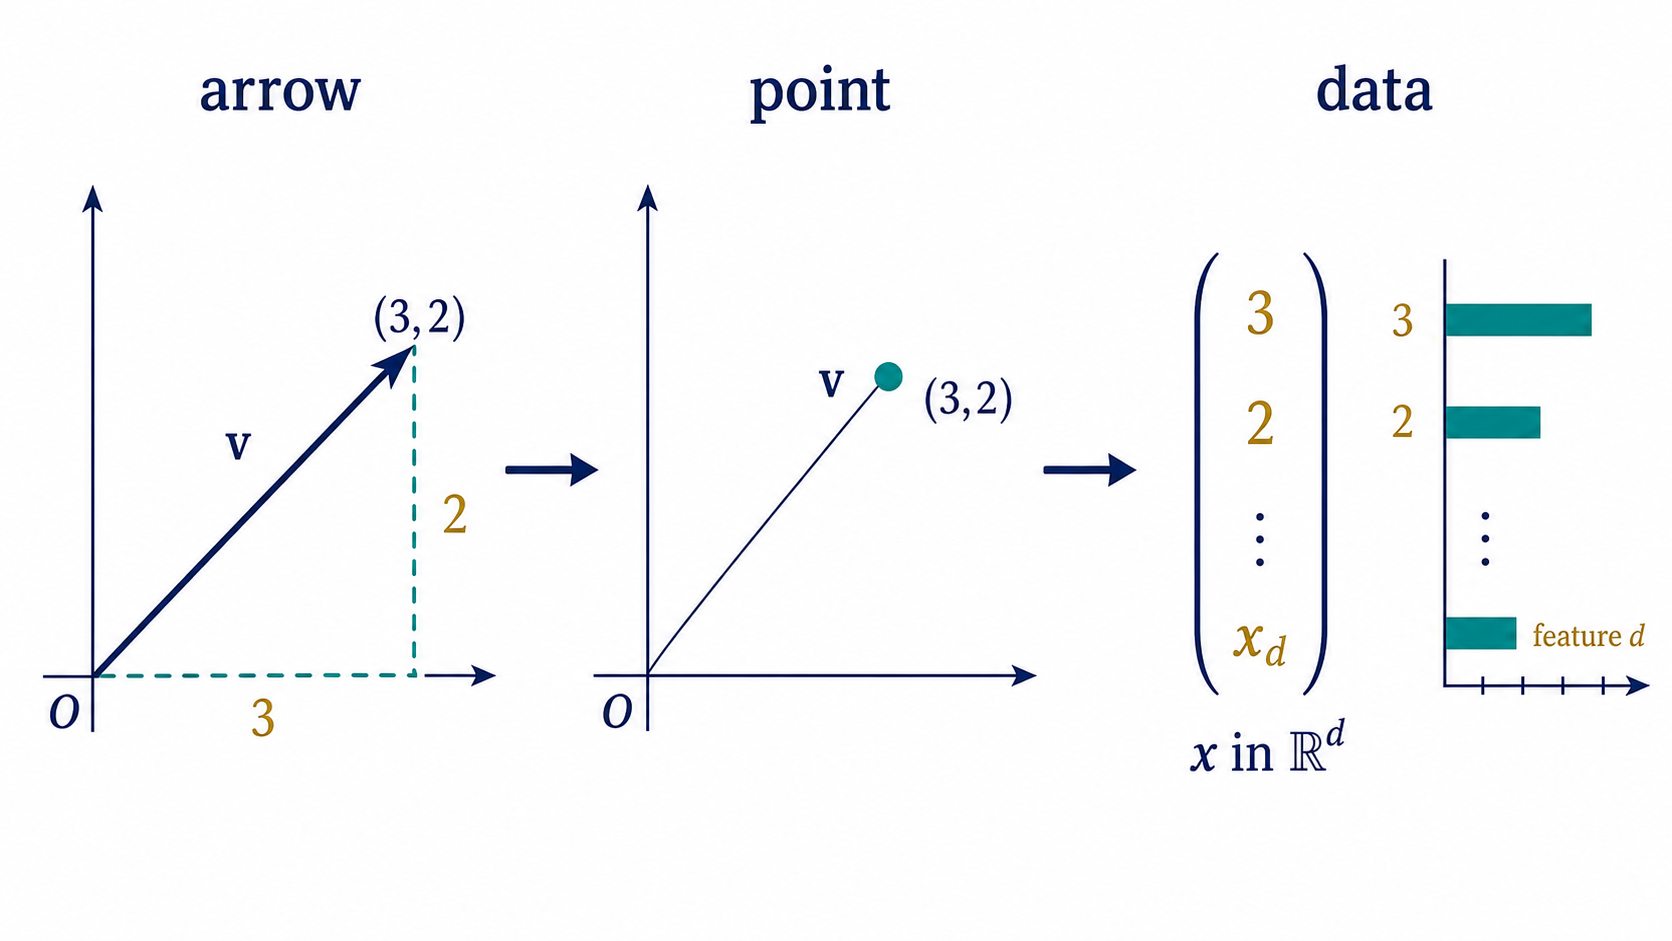
\includegraphics[width=0.95\linewidth]{imagegen-figures/ch03-vectors-three-views-v2.png}
\caption{One coordinate list, three interpretations. The vector \(v=(3,2)\) can be drawn as a displacement arrow, used as the coordinates of a point, or stored as the first two entries of a data vector \(x\in\mathbb{R}^d\). The mathematics gives the same addition and scaling rules in all three views; the application determines what the coordinates measure.}
\label{fig:ch03-vectors-three-views}
\end{figure}

\paragraph{Formal setup.}
For a positive integer \(d\), define
\[
\mathbb{R}^d=\{(v_1,\dots,v_d):v_i\in\mathbb{R}\text{ for }i=1,\dots,d\}.
\]
The standard coordinate vectors are
\[
e_1=(1,0,\dots,0),\quad e_2=(0,1,0,\dots,0),\quad \dots,\quad e_d=(0,\dots,0,1).
\]
Every vector \(v\in\mathbb{R}^d\) has the coordinate expansion
\[
v=v_1e_1+\cdots+v_de_d.
\]
If \(u,v\in\mathbb{R}^d\) and \(a\in\mathbb{R}\), vector addition and scalar multiplication are defined componentwise:
\[
u+v=\begin{bmatrix}u_1+v_1\\ \vdots\\ u_d+v_d\end{bmatrix},
\qquad
av=\begin{bmatrix}av_1\\ \vdots\\ av_d\end{bmatrix}.
\]
For data, it is common to collect \(n\) observations as rows of a matrix \(X\in\mathbb{R}^{n\times d}\), where row \(x_i\in\mathbb{R}^d\) is the vector of features for observation \(i\).

\paragraph{Core intuition.}
The arrow view makes addition visual. To add \(u+v\), place the tail of \(v\) at the head of \(u\); the resulting arrow goes from the original tail to the final head. The point view makes vectors feel like locations in a coordinate space. The data view makes vectors feel like records: one point in a space whose axes are measured features. Figure~\ref{fig:ch03-vectors-three-views} shows these three views side by side.

Common misconceptions come from mixing the views carelessly. First, an arrow vector is not tied to one position in the plane; the displacement \((3,2)\) can be drawn anywhere as long as its length and direction are unchanged. Second, a point vector does depend on an origin; moving the origin changes point coordinates. Third, a data vector's axes need not be spatial axes. Coordinate 17 might be a neuron's firing rate, a pixel intensity, or an embedding dimension.

This section extends Chapter 2's coordinate systems: a vector is an object with coordinates, not merely a tuple floating without context. It prepares Chapter 4, where matrices become functions that transform vectors, and Chapter 5, where projections split vectors into fitted and residual parts.

\paragraph{Main derivation: component rules from standard coordinates.}
If
\[
u=\sum_{i=1}^d u_i e_i,
\qquad
v=\sum_{i=1}^d v_i e_i,
\]
then
\[
u+v=\sum_{i=1}^d (u_i+v_i)e_i
\qquad\text{and}\qquad
av=\sum_{i=1}^d (av_i)e_i.
\]

\emph{Derivation.} Start with the coordinate expansions:
\[
u+v=\left(\sum_{i=1}^d u_i e_i\right)+\left(\sum_{i=1}^d v_i e_i\right).
\]
Addition lets us collect terms that point in the same coordinate direction:
\[
u+v=\sum_{i=1}^d u_i e_i+\sum_{i=1}^d v_i e_i.
\]
For each \(i\), both \(u_i e_i\) and \(v_i e_i\) lie along the same axis \(e_i\), so their coefficients add:
\[
u_i e_i+v_i e_i=(u_i+v_i)e_i.
\]
Putting this together gives \(u+v=\sum_i (u_i+v_i)e_i\). Scalar multiplication works the same way:
\[
av=a\sum_{i=1}^d v_i e_i=\sum_{i=1}^d (av_i)e_i.
\]
The mechanism is important: coordinates are weights on basis directions, and vector arithmetic updates those weights direction by direction.

\paragraph{Worked examples.}
\emph{Small numerical example.} Let
\[
u=\begin{bmatrix}1\\4\\-2\end{bmatrix},
\qquad
v=\begin{bmatrix}3\\-1\\5\end{bmatrix}.
\]
Then
\[
u+v=\begin{bmatrix}4\\3\\3\end{bmatrix},
\qquad
2u-v=
\begin{bmatrix}2\\8\\-4\end{bmatrix}
-
\begin{bmatrix}3\\-1\\5\end{bmatrix}
=
\begin{bmatrix}-1\\9\\-9\end{bmatrix}.
\]
Each coordinate is computed independently, but the result is a single geometric or data object.

\emph{Conceptual ML/neuroscience example.} Suppose a trial in a neural recording is
\[
x=\begin{bmatrix}12\\5\\0\\8\end{bmatrix}\in\mathbb{R}^4,
\]
where coordinate \(j\) is the spike count of neuron \(j\) in a time window. The mean response over many trials is also a vector. Subtracting the mean gives a deviation vector that points from baseline activity toward this trial's activity pattern. In representation learning, an embedding vector plays the same mathematical role: its coordinates are learned features rather than directly measured neurons.

\paragraph{ML/DL/neuroscience connections.}
In ML, a feature vector \(x\in\mathbb{R}^d\) is one input to a model. In deep learning, hidden activations are vectors whose coordinates are units or channels. In transformers, token embeddings and residual-stream states are high-dimensional vectors. In computational neuroscience, a population response vector has one coordinate per neuron, per time bin, or per latent factor. Later, gradients will be vectors in parameter space, covariance will summarize clouds of data vectors, and neural manifolds will be low-dimensional geometric sets inside high-dimensional population spaces.

\paragraph{Exercises.}
\begin{enumerate}[label=\textbf{3.1.\arabic*.}, leftmargin=*]
\item \textbf{Mechanical.} For \(u=(2,-1,4)\) and \(v=(-3,5,1)\), compute \(u+v\), \(3u\), and \(v-2u\).
\item \textbf{Proof or derivation.} Using \(e_1,\dots,e_d\), prove that the zero vector \(0=(0,\dots,0)\) satisfies \(v+0=v\) for every \(v\in\mathbb{R}^d\).
\item \textbf{Numerical/computational.} A data matrix \(X\in\mathbb{R}^{4\times 3}\) has rows \(x_1,\dots,x_4\). Write pseudocode that subtracts the row mean vector \(\bar x=\frac14\sum_i x_i\) from every row.
\item \textbf{Interpretation.} In a population response vector with one coordinate per neuron, what does the vector \(x-\bar x\) represent geometrically and experimentally?
\item \textbf{Debug the misconception.} A student says, ``The vector \((3,2)\) is always a physical arrow in the plane.'' Explain why this is too narrow and give two non-spatial interpretations.
\end{enumerate}

\subsection{3.2 Vector spaces and subspaces}

\paragraph{Motivating question.}
Which collections of vectors are stable enough that adding two allowed vectors, or rescaling an allowed vector, always keeps us inside the same collection?

\paragraph{Beginner setup.}
A \emph{vector space} is a set of objects that can be added and scaled while obeying the usual algebraic laws. The objects do not have to be arrows in the plane. They may be lists of numbers, images, functions, signals, or parameter vectors. A \emph{subspace} is a smaller vector space living inside a larger one.

The smallest nontrivial example is a line through the origin in \(\mathbb{R}^2\):
\[
W=\{a(1,2):a\in\mathbb{R}\}.
\]
Adding two vectors on this line gives another vector on the line:
\[
a(1,2)+b(1,2)=(a+b)(1,2).
\]
Scaling a vector on the line keeps it on the line:
\[
c\,a(1,2)=(ca)(1,2).
\]
By contrast, the line \(\{(1,0)+a(1,2):a\in\mathbb{R}\}\) is not a subspace because it misses the origin and is not closed under scaling.

Vector spaces solve the problem of legitimate linear combination. If a model assumes the allowed states form a subspace, then mixtures, averages, contrasts, and directions all remain meaningful inside that model.

What to keep in mind: a subspace is not just any geometric shape inside a vector space. It must contain the zero vector and be closed under all linear combinations. A spanning list tells us how to generate a subspace; a basis tells us how to describe every vector in that subspace without redundancy.

\begin{figure}[htbp]
\centering
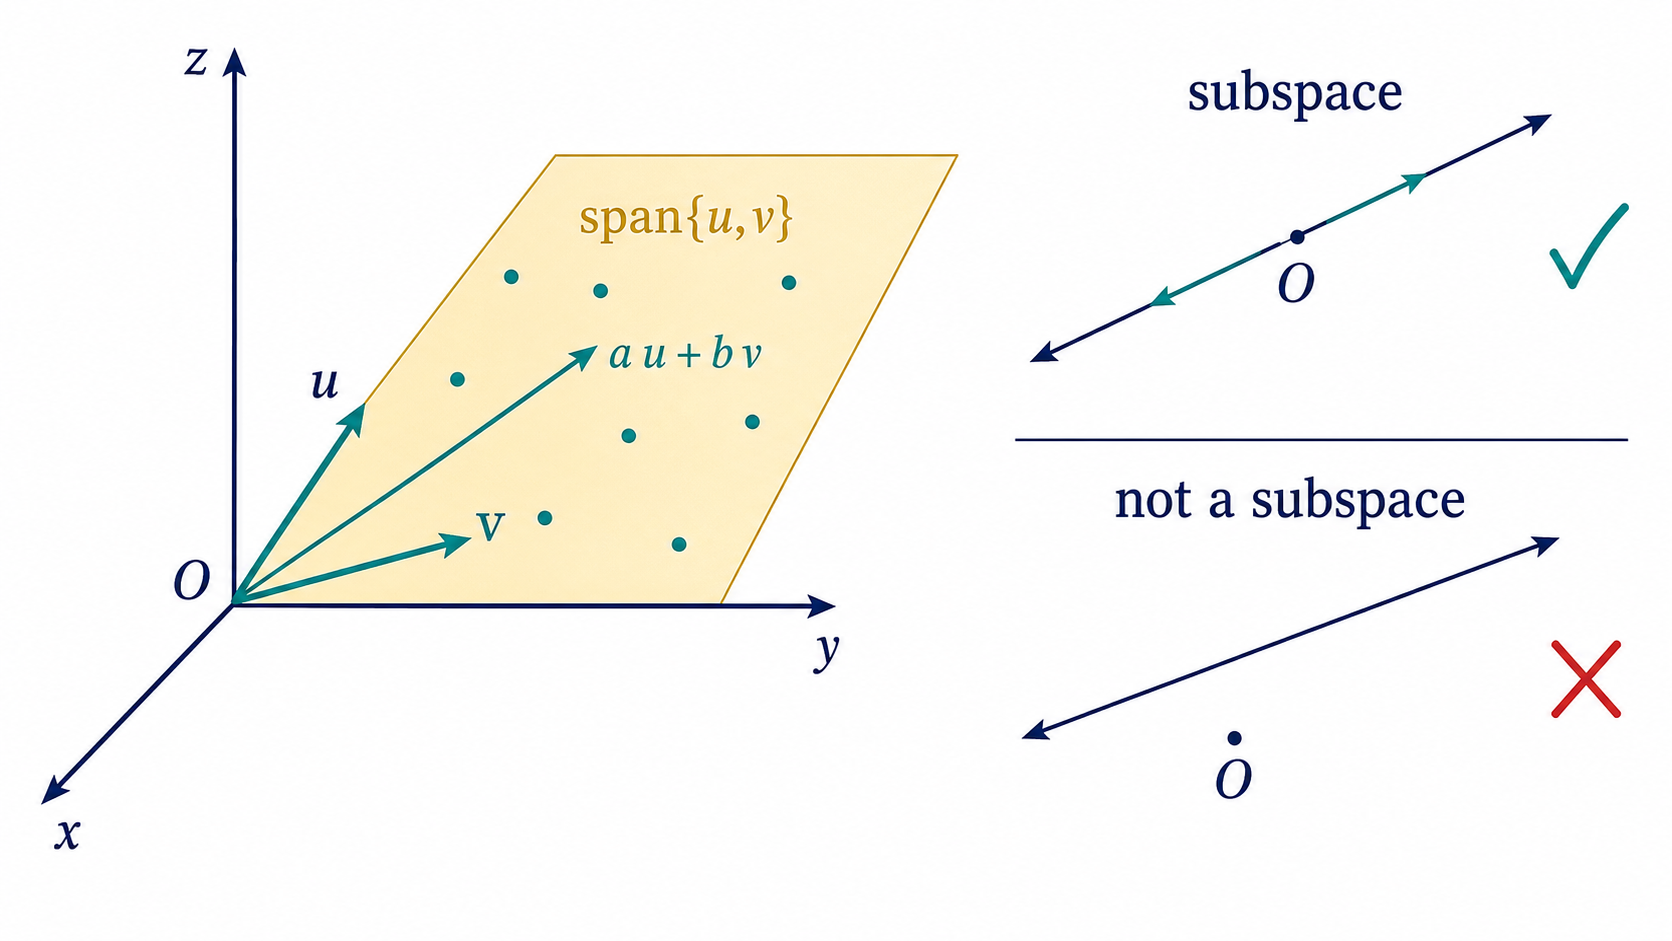
\includegraphics[width=0.95\linewidth]{imagegen-figures/ch03-span-subspaces.png}
\caption{Span and subspace structure. The plane \(\operatorname{span}\{u,v\}\) contains all linear combinations \(au+bv\) and passes through the origin. A line through the origin is a subspace; a parallel offset line is not, because it fails the zero-vector and scaling tests.}
\label{fig:ch03-span-subspaces}
\end{figure}

\paragraph{Formal setup.}
Let \(V\) be a set with addition \(+:V\times V\to V\) and scalar multiplication \(\mathbb{R}\times V\to V\). We call \(V\) a real vector space when these operations satisfy the standard laws: associativity and commutativity of addition, existence of a zero vector and additive inverses, distributivity over vector addition and scalar addition, compatibility of scalar multiplication, and \(1v=v\).

A subset \(W\subseteq V\) is a \emph{subspace} if \(W\) is itself a vector space using the same addition and scalar multiplication. Equivalently, \(W\) is nonempty and for all \(u,v\in W\) and all \(a,b\in\mathbb{R}\),
\[
au+bv\in W.
\]
Given vectors \(v_1,\dots,v_k\in V\), their \emph{span} is
\[
\operatorname{span}\{v_1,\dots,v_k\}
=\{a_1v_1+\cdots+a_kv_k:a_1,\dots,a_k\in\mathbb{R}\}.
\]
The coefficients \(a_i\) are scalars; the output is a vector in \(V\).

A list \(v_1,\dots,v_k\) is \emph{linearly independent} if the only way to make the zero vector is the trivial combination
\[
a_1v_1+\cdots+a_kv_k=0
\quad\Longrightarrow\quad
a_1=\cdots=a_k=0.
\]
If a list spans a subspace \(W\) and is linearly independent, it is a \emph{basis} for \(W\). In this chapter we work with finite-dimensional subspaces: when \(W\) has a finite basis, the number of vectors in any basis for \(W\) is the \emph{dimension} of \(W\), written \(\dim W\). Thus a line through the origin has dimension \(1\), a plane through the origin has dimension \(2\), and \(\mathbb{R}^d\) has dimension \(d\).

\paragraph{Core intuition.}
Span is the set of all destinations reachable by moving along a chosen list of directions with arbitrary real step sizes. One nonzero vector spans a line through the origin. Two non-collinear vectors in \(\mathbb{R}^3\) span a plane through the origin. Three suitable vectors span all of \(\mathbb{R}^3\). Figure~\ref{fig:ch03-span-subspaces} makes the closure idea visible: once \(u\) and \(v\) are allowed, every \(au+bv\) must be allowed.

The most common misconception is that a subspace is any line, plane, or cluster-like region. A line in \(\mathbb{R}^2\) is a subspace only if it passes through the origin. A plane in \(\mathbb{R}^3\) is a subspace only if it passes through the origin. A curved manifold, a sphere, or a probability simplex may have useful geometry, but it is not a vector subspace under ordinary addition and scaling. Another common confusion is to treat every spanning list as a basis. A spanning list may contain redundant directions; a basis is a spanning list with no redundant direction.

This section depends on Chapter 2's algebraic structures: the operations define the object. It points forward to column spaces and null spaces of matrices, feature subspaces, linear models, PCA subspaces, and low-dimensional neural activity subspaces.

\paragraph{Main theorem: span is the smallest subspace containing the generators.}
For vectors \(v_1,\dots,v_k\in V\), the set \(\operatorname{span}\{v_1,\dots,v_k\}\) is a subspace of \(V\). Moreover, it is the smallest subspace containing \(v_1,\dots,v_k\): if \(U\subseteq V\) is any subspace with \(v_1,\dots,v_k\in U\), then
\[
\operatorname{span}\{v_1,\dots,v_k\}\subseteq U.
\]

\emph{Proof sketch.} First show that the span is closed. Take two vectors in the span:
\[
x=a_1v_1+\cdots+a_kv_k,
\qquad
y=b_1v_1+\cdots+b_kv_k.
\]
For scalars \(\alpha,\beta\), form the linear combination
\[
\alpha x+\beta y
=\alpha\sum_{i=1}^k a_i v_i+\beta\sum_{i=1}^k b_i v_i.
\]
Distributing the scalars through the sums gives
\[
\alpha x+\beta y
=\sum_{i=1}^k \alpha a_i v_i+\sum_{i=1}^k \beta b_i v_i.
\]
Terms in the same generator \(v_i\) can be collected:
\[
\alpha x+\beta y
=\sum_{i=1}^k (\alpha a_i+\beta b_i)v_i.
\]
This is again a linear combination of \(v_1,\dots,v_k\), so it lies in the span.

Now suppose \(U\) is any subspace containing every \(v_i\). Because \(U\) is closed under scaling, \(a_i v_i\in U\). Because \(U\) is closed under addition, every sum \(a_1v_1+\cdots+a_kv_k\) lies in \(U\). Thus every vector in the span lies in \(U\). The span is therefore the smallest subspace forced by the generators.

\paragraph{Worked examples.}
\emph{Small numerical example.} In \(\mathbb{R}^3\), let
\[
u=(1,0,1),\qquad v=(0,1,1).
\]
Then
\[
\operatorname{span}\{u,v\}
=\{a(1,0,1)+b(0,1,1):a,b\in\mathbb{R}\}
=\{(a,b,a+b):a,b\in\mathbb{R}\}.
\]
This is the plane \(z=x+y\), and it passes through the origin. The vectors \(u\) and \(v\) are linearly independent: if
\[
au+bv=(a,b,a+b)=(0,0,0),
\]
then \(a=0\) and \(b=0\). Therefore \(\{u,v\}\) is a basis for this plane and the plane has dimension \(2\). The vector \((2,-1,1)\) lies in the span because \(1=2+(-1)\). The vector \((2,-1,4)\) does not.

\emph{Conceptual ML/neuroscience example.} In a linear model, predictions have the form
\[
\hat y=w_1x^{(1)}+\cdots+w_dx^{(d)},
\]
where \(x^{(j)}\in\mathbb{R}^n\) is the \(j\)th feature column across \(n\) examples. All possible predictions lie in the span of the feature columns. In neural population analysis, a task subspace may be spanned by a few directions corresponding to stimulus, choice, or movement. Projecting activity into that span asks how much of the population response is explainable by those task directions.

\paragraph{ML/DL/neuroscience connections.}
The column space of a data matrix is a subspace of possible linear predictions. The null space of a matrix is the subspace of inputs invisible to a linear map. In deep networks, a layer's activations often concentrate near a low-dimensional subspace or manifold inside a high-dimensional ambient space. In neuroscience, population activity during a task may occupy a subspace whose axes correspond to latent dynamics, task variables, or preparatory states. Later, PCA will choose a subspace that captures maximal variance, while least squares will find the closest vector inside a prediction subspace.

\paragraph{Exercises.}
\begin{enumerate}[label=\textbf{3.2.\arabic*.}, leftmargin=*]
\item \textbf{Mechanical.} Decide whether each set is a subspace of \(\mathbb{R}^2\): \(W_1=\{(a,2a):a\in\mathbb{R}\}\), \(W_2=\{(1,a):a\in\mathbb{R}\}\), and \(W_3=\{(x,y):x+y=0\}\).
\item \textbf{Proof or derivation.} Prove the subspace test: a nonempty subset \(W\subseteq V\) is a subspace if and only if \(au+bv\in W\) for all \(u,v\in W\) and all \(a,b\in\mathbb{R}\).
\item \textbf{Numerical/computational.} Given \(u=(1,2,0)\), \(v=(0,1,1)\), and \(w=(3,7,2)\), solve for \(a,b\) such that \(w=au+bv\), or show that no solution exists. Then decide whether \(\{u,v\}\) is a basis for its span and state the dimension of that span.
\item \textbf{Interpretation.} If all predictions of a linear regression model lie in the span of the feature columns, what does it mean for the target vector \(y\) to lie outside that span?
\item \textbf{Debug the misconception.} A student says, ``The set of all probability vectors in \(\mathbb{R}^3\) is a subspace because it is a flat triangle.'' Explain which vector-space operations fail.
\end{enumerate}

\subsection{3.3 Norms, distances, and angles}

\paragraph{Motivating question.}
How do we turn vectors into quantitative statements about size, separation, and directional similarity?

\paragraph{Beginner setup.}
A \emph{norm} assigns a nonnegative length \(\|x\|\) to a vector \(x\). A \emph{distance} assigns a separation \(d(x,y)\) to two points. An \emph{angle} measures how directions align. These are related but not identical ideas:
\[
\text{size from origin: }\|x\|,
\qquad
\text{separation: }d(x,y)=\|x-y\|,
\qquad
\text{alignment: }\cos\theta=\frac{\langle x,y\rangle}{\|x\|\|y\|}.
\]

The smallest nontrivial example is \(x=(3,4)\). Its Euclidean norm is
\[
\|x\|_2=\sqrt{3^2+4^2}=5.
\]
If \(y=(6,8)\), then \(d(x,y)=\|y-x\|_2=\|(3,4)\|_2=5\), even though \(y\) itself is farther from the origin. Norm measures one vector; distance measures a difference between two vectors.

Norms, distances, and angles solve the problem of comparison. They let us define nearest neighbors, similarity, error size, regularization penalties, convergence, and geometric learning objectives.

What to keep in mind: there is no single universal notion of size. \(\ell_2\) length, \(\ell_1\) length, cosine similarity, and correlation emphasize different structure. Choosing a geometry is a modeling decision.

\begin{figure}[htbp]
\centering
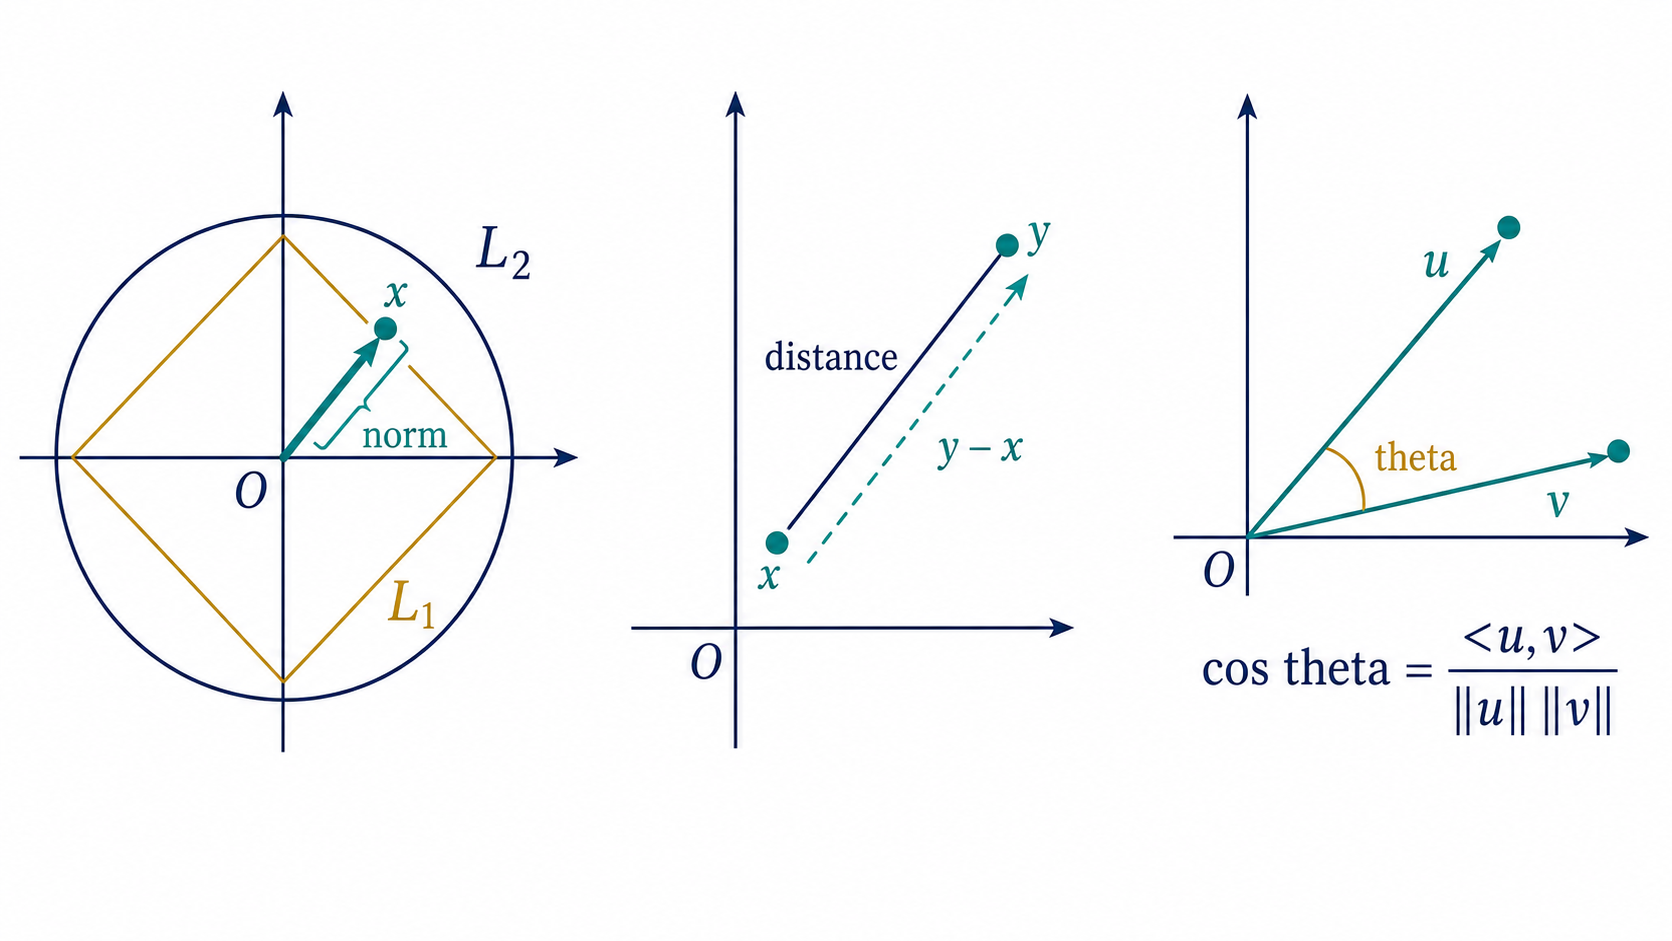
\includegraphics[width=0.95\linewidth]{imagegen-figures/ch03-norms-distances-angles.png}
\caption{Three measurements on vectors. A norm measures size relative to the origin and depends on the chosen unit ball, such as the circular \(\ell_2\) ball or diamond-shaped \(\ell_1\) ball. A distance is the norm of a difference \(y-x\). An angle compares directions through the normalized inner product.}
\label{fig:ch03-norms-distances-angles}
\end{figure}

\paragraph{Formal setup.}
A norm on a real vector space \(V\) is a function \(\|\cdot\|:V\to\mathbb{R}_{\ge 0}\) satisfying, for all \(x,y\in V\) and \(a\in\mathbb{R}\),
\[
\|x\|=0\iff x=0,\qquad
\|ax\|=|a|\|x\|,\qquad
\|x+y\|\le \|x\|+\|y\|.
\]
On \(\mathbb{R}^d\), common examples are
\[
\|x\|_2=\left(\sum_{i=1}^d x_i^2\right)^{1/2},
\qquad
\|x\|_1=\sum_{i=1}^d |x_i|,
\qquad
\|x\|_\infty=\max_i |x_i|.
\]
The Euclidean inner product is
\[
\langle x,y\rangle=\sum_{i=1}^d x_i y_i.
\]
For nonzero \(x,y\in\mathbb{R}^d\), the Euclidean angle \(\theta\in[0,\pi]\) is defined by
\[
\cos\theta=\frac{\langle x,y\rangle}{\|x\|_2\|y\|_2}.
\]

\paragraph{Core intuition.}
A norm is defined by its unit ball: the set of vectors counted as length at most one. The Euclidean unit ball is round; all directions are treated equally. The \(\ell_1\) unit ball is a diamond in two dimensions; it favors coordinate-axis sparsity in optimization. Distance translates the picture: the distance from \(x\) to \(y\) is the length of the arrow from \(x\) to \(y\). Angle ignores scale and asks whether two nonzero vectors point in similar directions. Figure~\ref{fig:ch03-norms-distances-angles} separates these three measurements.

Common misconceptions: a large dot product does not necessarily mean a small angle, because the dot product grows with vector lengths. Cosine similarity corrects for this by dividing by the norms. Another misconception is that small Euclidean distance always means semantic similarity. In high-dimensional ML, distance depends strongly on representation, scaling, and preprocessing. Finally, \(\ell_1\) and \(\ell_2\) are not interchangeable: they produce different optimization geometry.

This section builds on vector arithmetic from Section 3.1 and prepares projections in Section 3.4. Later, norms will define losses, regularizers, convergence criteria, adversarial perturbation budgets, and probability metrics.

\paragraph{Main theorem: Cauchy--Schwarz makes the angle formula valid.}
For all \(x,y\in\mathbb{R}^d\),
\[
|\langle x,y\rangle|\le \|x\|_2\|y\|_2.
\]
Therefore, for nonzero \(x,y\),
\[
-1\le \frac{\langle x,y\rangle}{\|x\|_2\|y\|_2}\le 1,
\]
so the angle formula defines a valid cosine value.

\emph{Proof sketch.} If \(y=0\), both sides are zero. Assume \(y\ne 0\). For any real \(t\), the squared length of \(x-ty\) is nonnegative:
\[
0\le \|x-ty\|_2^2.
\]
Expand the square using the inner product:
\[
\|x-ty\|_2^2=\langle x-ty,x-ty\rangle.
\]
Bilinearity of the inner product gives
\[
\langle x-ty,x-ty\rangle
=\langle x,x\rangle-2t\langle x,y\rangle+t^2\langle y,y\rangle.
\]
Rewrite lengths as norms:
\[
\|x-ty\|_2^2=\|x\|_2^2-2t\langle x,y\rangle+t^2\|y\|_2^2.
\]
This quadratic in \(t\) is never negative. Its best choice of \(t\) is the one that minimizes the quadratic:
\[
t^\star=\frac{\langle x,y\rangle}{\|y\|_2^2}.
\]
Substituting \(t^\star\) leaves
\[
0\le \|x\|_2^2-\frac{\langle x,y\rangle^2}{\|y\|_2^2}.
\]
Multiplying by \(\|y\|_2^2>0\) gives
\[
\langle x,y\rangle^2\le \|x\|_2^2\|y\|_2^2.
\]
Taking square roots gives Cauchy--Schwarz. The mechanism is geometric: the closest multiple of \(y\) to \(x\) cannot make a negative squared residual, and that fact bounds the possible dot product.

\paragraph{Worked examples.}
\emph{Small numerical example.} Let \(x=(1,2,2)\) and \(y=(2,0,1)\). Then
\[
\|x\|_2=3,\qquad \|y\|_2=\sqrt5,\qquad \langle x,y\rangle=4.
\]
The cosine of the angle is
\[
\cos\theta=\frac{4}{3\sqrt5}\approx 0.596.
\]
The vectors are positively aligned but not close to parallel. Their Euclidean distance is
\[
\|x-y\|_2=\|(-1,2,1)\|_2=\sqrt6.
\]

\emph{Conceptual ML/neuroscience example.} In embedding models, cosine similarity compares directions rather than lengths. Two token embeddings can have high cosine similarity if they point in similar representational directions, even if one has larger norm. In neural data, the angle between two population response vectors can measure whether two stimuli recruit similar response patterns across neurons; the norm measures response magnitude, and distance measures trial-to-trial or condition-to-condition separation.

\paragraph{ML/DL/neuroscience connections.}
Mean-squared error uses the squared \(\ell_2\) norm of residuals. Lasso regularization uses the \(\ell_1\) norm to encourage sparse coefficients. Contrastive and retrieval models often compare normalized embeddings by cosine similarity. Adversarial robustness studies perturbations constrained by \(\ell_2\), \(\ell_\infty\), or other norms. In neuroscience, population-vector length can reflect response strength, distances can quantify discriminability between conditions, and angles can reveal whether two tasks use aligned or rotated neural subspaces.

\paragraph{Exercises.}
\begin{enumerate}[label=\textbf{3.3.\arabic*.}, leftmargin=*]
\item \textbf{Mechanical.} For \(x=(-2,1,2)\), compute \(\|x\|_1\), \(\|x\|_2\), and \(\|x\|_\infty\).
\item \textbf{Proof or derivation.} Use Cauchy--Schwarz to prove the Euclidean triangle inequality \(\|x+y\|_2\le \|x\|_2+\|y\|_2\).
\item \textbf{Numerical/computational.} Write pseudocode that takes two nonzero vectors and returns their cosine similarity. Include a check for zero norm.
\item \textbf{Interpretation.} Two neural population vectors have large norms but cosine similarity near zero. What does that say about response magnitude and response pattern?
\item \textbf{Debug the misconception.} A student says, ``The largest dot product always means the most similar vector.'' Explain why vector length can make this false and how cosine similarity changes the comparison.
\end{enumerate}

\subsection{3.4 Orthogonality and decomposition}

\paragraph{Motivating question.}
How can we split a vector into the part explained by a chosen direction or subspace and the leftover part that is perpendicular to it?

\paragraph{Beginner setup.}
Two vectors \(u,v\in\mathbb{R}^d\) are \emph{orthogonal} if
\[
\langle u,v\rangle=0.
\]
Geometrically, they meet at a right angle. A \emph{decomposition} writes one vector as a sum of meaningful pieces. The most important beginner decomposition is
\[
x=p+r,
\]
where \(p\) lies in a subspace \(W\) and \(r\) is orthogonal to every vector in \(W\). The vector \(p\) is the projection of \(x\) onto \(W\), and \(r\) is the residual.

The smallest nontrivial example is projection onto a line. Let \(W=\operatorname{span}\{u\}\), where \(u\ne 0\). The part of \(x\) along the line is
\[
p=\frac{\langle x,u\rangle}{\langle u,u\rangle}u.
\]
The residual is \(r=x-p\), and it satisfies \(\langle r,u\rangle=0\).

Orthogonal decomposition solves the problem of best linear explanation. It tells us how much of \(x\) is captured by a direction or subspace and how much remains unexplained.

What to keep in mind: orthogonal does not mean unrelated in every possible sense. It means zero inner product under the chosen geometry. Change the inner product or preprocessing, and orthogonality can change.

\begin{figure}[htbp]
\centering
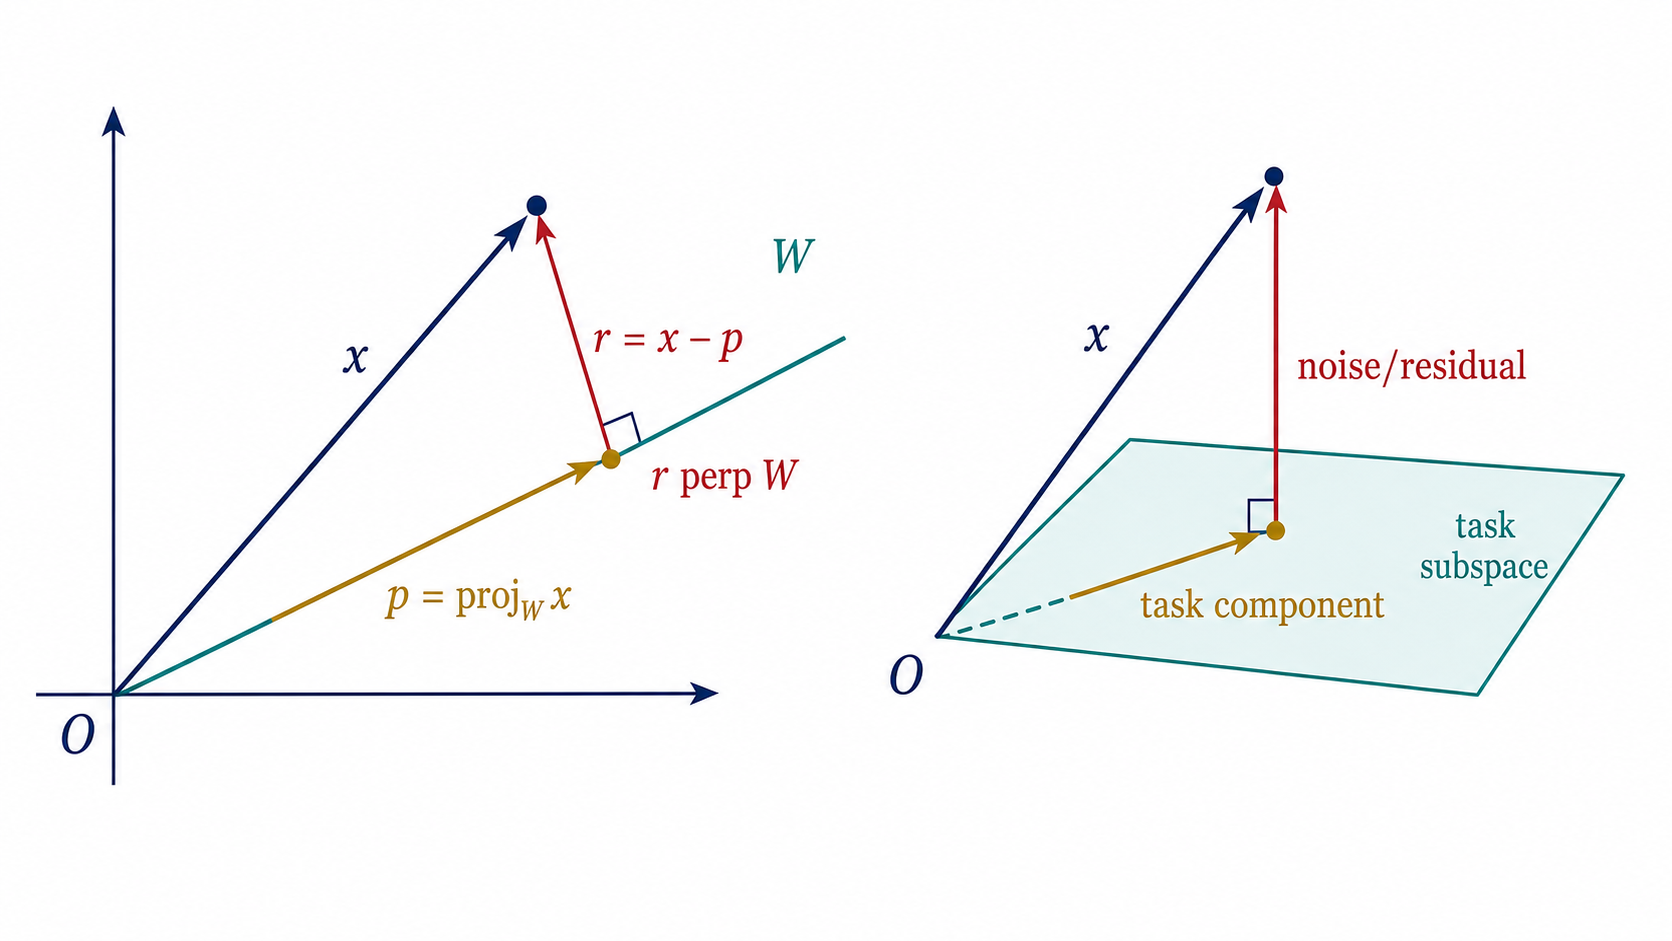
\includegraphics[width=0.95\linewidth]{imagegen-figures/ch03-orthogonal-decomposition.png}
\caption{Orthogonal decomposition as explained part plus residual. The projection \(p=\operatorname{proj}_W x\) lies inside the subspace \(W\). The residual \(r=x-p\) points from the projection to \(x\) and is perpendicular to \(W\). In neural population geometry, the same picture separates a task component from residual activity outside the task subspace.}
\label{fig:ch03-orthogonal-decomposition}
\end{figure}

\paragraph{Formal setup.}
For a subspace \(W\subseteq\mathbb{R}^d\), the orthogonal complement is
\[
W^\perp=\{z\in\mathbb{R}^d:\langle z,w\rangle=0\text{ for every }w\in W\}.
\]
An \emph{orthonormal basis} for \(W\) is a list \(q_1,\dots,q_k\in W\) such that
\[
\langle q_i,q_j\rangle=
\begin{cases}
1,& i=j,\\
0,& i\ne j.
\end{cases}
\]
If \(q_1,\dots,q_k\) is an orthonormal basis for \(W\), the projection of \(x\in\mathbb{R}^d\) onto \(W\) is
\[
\operatorname{proj}_W x=\sum_{j=1}^k \langle x,q_j\rangle q_j.
\]
The residual is
\[
r=x-\operatorname{proj}_W x.
\]

\paragraph{Core intuition.}
Projection drops a perpendicular from \(x\) to the subspace \(W\). The landing point is the closest point in \(W\). The residual is the arrow from that landing point back to \(x\). Figure~\ref{fig:ch03-orthogonal-decomposition} shows this in two views: a line subspace in the plane and a task subspace inside neural population space.

Common misconceptions: first, projection is not the same as deleting coordinates unless the subspace is aligned with coordinate axes. Second, a residual being orthogonal to \(W\) does not mean it is unimportant; it means it is not captured by the chosen subspace. Third, orthogonality depends on the inner product. In a weighted geometry, the projection formula changes.

This section builds directly on Sections 3.2 and 3.3: subspaces give the allowed explanatory set, and inner products define perpendicularity. It leads into Chapter 5, where least squares is exactly projection onto a column space, and into Chapter 6, where PCA chooses orthogonal directions of maximal variance.

\paragraph{Main theorem: orthogonal decomposition onto a finite-dimensional subspace.}
Let \(W\subseteq\mathbb{R}^d\) be a subspace with orthonormal basis \(q_1,\dots,q_k\). For every \(x\in\mathbb{R}^d\), define
\[
p=\sum_{j=1}^k \langle x,q_j\rangle q_j,
\qquad
r=x-p.
\]
Then \(p\in W\), \(r\in W^\perp\), and \(x=p+r\). This decomposition is unique. Moreover, \(p\) is the closest vector in \(W\) to \(x\):
\[
\|x-p\|_2\le \|x-w\|_2
\qquad\text{for all }w\in W.
\]

\emph{Proof sketch.} The vector \(p\) is a linear combination of \(q_1,\dots,q_k\), so \(p\in W\). The identity \(x=p+r\) is true by the definition \(r=x-p\). The key point is orthogonality. For each basis vector \(q_i\),
\[
\langle r,q_i\rangle
=\left\langle x-\sum_{j=1}^k \langle x,q_j\rangle q_j,\ q_i\right\rangle.
\]
Distribute the inner product over subtraction and the sum:
\[
\langle r,q_i\rangle
=\langle x,q_i\rangle-\sum_{j=1}^k \langle x,q_j\rangle\langle q_j,q_i\rangle.
\]
Because the basis is orthonormal, \(\langle q_j,q_i\rangle=0\) when \(j\ne i\) and equals \(1\) when \(j=i\). The sum therefore collapses to the single term \(\langle x,q_i\rangle\):
\[
\langle r,q_i\rangle=\langle x,q_i\rangle-\langle x,q_i\rangle=0.
\]
Since \(r\) is orthogonal to every basis direction, it is orthogonal to every vector in \(W\).

To prove closest-point behavior, take any \(w\in W\). Then \(p-w\in W\), while \(r\in W^\perp\). Thus \(r\) and \(p-w\) are orthogonal. By the Pythagorean theorem,
\[
\|x-w\|_2^2=\|(p+r)-w\|_2^2
=\|r+(p-w)\|_2^2
=\|r\|_2^2+\|p-w\|_2^2.
\]
The second term is nonnegative, so \(\|x-w\|_2^2\ge \|r\|_2^2=\|x-p\|_2^2\). Therefore \(p\) is closest. Uniqueness follows because two decompositions would subtract to a vector lying in both \(W\) and \(W^\perp\), and only the zero vector can do that.

\paragraph{Worked examples.}
\emph{Small numerical example.} Let \(x=(2,3)\) and let \(W=\operatorname{span}\{u\}\) with \(u=(1,1)\). The projection onto the line is
\[
p=\frac{\langle x,u\rangle}{\langle u,u\rangle}u
=\frac{5}{2}(1,1)
=\left(\frac52,\frac52\right).
\]
The residual is
\[
r=x-p=\left(-\frac12,\frac12\right).
\]
Check orthogonality:
\[
\langle r,u\rangle=-\frac12+\frac12=0.
\]
Thus \(x\) has been split into its component along the diagonal line and a perpendicular leftover.

\emph{Conceptual ML/neuroscience example.} In least-squares regression, the target vector \(y\in\mathbb{R}^n\) is decomposed into \(\hat y+r\), where \(\hat y\) lies in the column space of the design matrix \(X\), and the residual \(r=y-\hat y\) is orthogonal to every feature column. In neural population analysis, a task subspace \(W\) may be spanned by movement-related directions. Projecting a trial vector \(x\) onto \(W\) gives the task component; the orthogonal residual contains activity not explained by those selected task variables.

\paragraph{ML/DL/neuroscience connections.}
Backpropagation computes gradient vectors, and optimization often decomposes updates into useful directions and constrained residuals. Least squares, linear decoding, and PCA are all projection stories. In representation analysis, orthogonal subspaces can separate stimulus, choice, context, and movement components when the geometry supports that interpretation. In modern AI systems, residual-stream analyses sometimes ask whether a feature direction, task vector, or steering vector explains a component of activation; mathematically, this is a projection and residual question.

\paragraph{Exercises.}
\begin{enumerate}[label=\textbf{3.4.\arabic*.}, leftmargin=*]
\item \textbf{Mechanical.} Project \(x=(4,1)\) onto \(W=\operatorname{span}\{(1,2)\}\). Compute the residual and verify orthogonality.
\item \textbf{Proof or derivation.} Prove that \(W^\perp\) is a subspace of \(\mathbb{R}^d\).
\item \textbf{Numerical/computational.} Suppose \(q_1=(1,0,0)\) and \(q_2=(0,1,0)\). Use the orthonormal-basis projection formula to project \(x=(2,-1,5)\) onto \(W=\operatorname{span}\{q_1,q_2\}\).
\item \textbf{Interpretation.} In a regression problem, what does it mean geometrically for the residual to be orthogonal to every feature column?
\item \textbf{Debug the misconception.} A student says, ``If the residual is orthogonal to the task subspace, it must be random noise.'' Explain why orthogonality to one chosen subspace does not imply randomness or irrelevance.
\end{enumerate}

\paragraph{Closing bridge.}
This chapter made coordinate lists geometric: vectors can be generated by bases, compared by lengths and angles, and decomposed by orthogonality. Chapter 4 keeps the same objects but asks what happens when a rule transforms every vector while preserving addition and scaling. That question turns vectors into the inputs and outputs of matrices. Chapter 5 then returns to the projection picture and makes it the core mechanism of least-squares fitting.

\clearpage
